\documentclass[tikz,border=10pt]{standalone}
\usepackage{amsmath}
\usepackage{tikz}
\usetikzlibrary{positioning}

\tikzset{
  card/.style={draw=blue!70!black, line width=1.2pt, rounded corners=3pt, minimum width=5.8cm, minimum height=4.5cm, align=left, fill=none}
}

\begin{document}
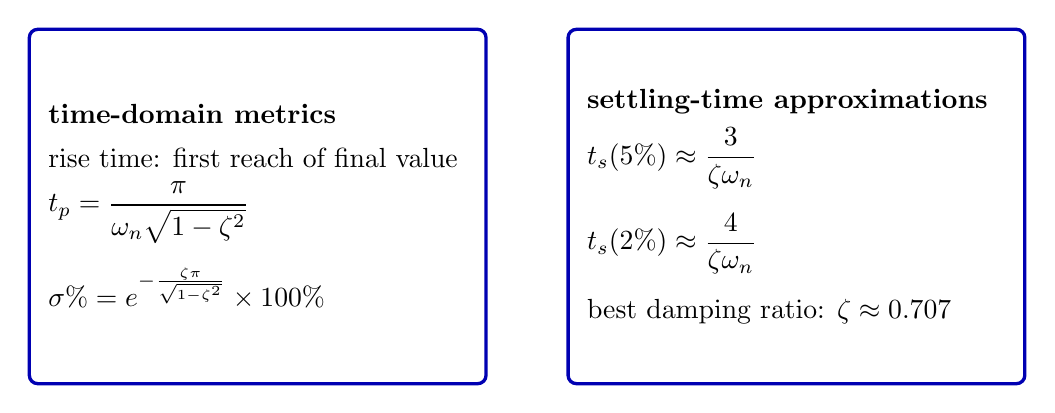
\begin{tikzpicture}[node distance=0.9cm]
  \node[card] (left) {
    \begin{minipage}{5.2cm}
      \textbf{time-domain metrics}\\[4pt]
      rise time: first reach of final value\\[4pt]
      $t_p=\dfrac{\pi}{\omega_n\sqrt{1-\zeta^2}}$\\[8pt]
      $\sigma\%=e^{-\frac{\zeta\pi}{\sqrt{1-\zeta^2}}}\times 100\%$
    \end{minipage}
  };
  \node[card, right=1.0cm of left] (right) {
    \begin{minipage}{5.2cm}
      \textbf{settling-time approximations}\\[4pt]
      $t_s(5\%) \approx \dfrac{3}{\zeta\omega_n}$\\[8pt]
      $t_s(2\%) \approx \dfrac{4}{\zeta\omega_n}$\\[8pt]
      best damping ratio: $\zeta \approx 0.707$
    \end{minipage}
  };
\end{tikzpicture}
\end{document}
